% Instructions to change to html version:
% Comment out:
%  minipage, multicols,columnbreak, mathbf, hrule
% Replace all: \begin{minipage}% \end{minipage} %\begin{mulicols}  %\end{mulicols}  %\columnbreak % \begin{framed} %\end{framed} %\hrule
% Search for \mathbf
% Replace \\] with \[ and \) with \(
% Enclose graphics in figure environments and add captions
% Re-tag \df environments as sections, subsections, etc.
% Command Line Code to Create html version:
%First: pdflatex -shell-escape filename.tex                                   
%Second, for each figure: inkscape "filename-figure1.pdf" -o "filename-figure1.png"
% Third: htlatex filename.tex "ht5mjlatex.cfg, charset=utf-8" " -cunihtf -utf8"

\documentclass[10pt]{article}

%\usepackage{tikz, pgf,pgfplots,wasysym,array}
%\usepackage{wasysym,array}

\usepackage{amsmath,amssymb}

\ifdefined\HCode
  \def\pgfsysdriver{pgfsys-tex4ht-updated.def}
\fi 
%\ifdefined\HCode
%  \def\pgfsysdriver{pgfsys-dvisvgm4ht.def}
%\fi 
\usepackage{tikz}
\usetikzlibrary{calc,decorations.markings,arrows}
\usepackage{pgfplots}

\pgfplotsset{compat=1.12}
\usepackage{myexternalize}
\usetikzlibrary{calc,decorations.markings,arrows}
\usepackage{framed}
\usepackage[none]{hyphenat}

\input{../../../common/1336_header_test.tex}
\begin{document}



\newcommand{\an}{\lbrace a_n \rbrace}
\newcommand{\Sum}{\sum_{n=1}^\infty }
\newcommand{\Sumzero}{\sum_{n=0}^\infty }

\everymath{\displaystyle}

\renewcommand{\myTitle}{	MATH 1336: Calculus III}

\renewcommand{\mySubTitle}{Section 8.7, Part 2: More Practice with Taylor \& Maclaurin Series}
%~\hfill Name: \underline{~~~~~~~~~~~~~~~~~~~~~~~~~~~~~~~~~~~~~~~~~~~~~~~}


%%% Spring 2023: Very short on time, so no error estimation, and remove the trickier two parts of problem 3. Also relabel as Taylor \& Maclaurin Practice Problems, since there probably will not be time for group work.

%\lectTitle{\vspace*{-.6in}\myTitle}{\vspace*{.1in}\mySubTitle \vspace*{-.4in}}


\title{\mySubTitle}\date{}
\maketitle


\hspace*{-.8in}%\begin{minipage}{1.25\textwidth}

\setlength{\columnseprule}{.4pt}
\setlength{\columnsep}{3em}

%\begin{framed}
\section*{Taylor/Maclaurin Series Summary:}
\textbf{\underline{\large Key Idea:}}
When \(x\) is close to \(a\) and \(n\) is large: the \(n^{th}\) degree Taylor/Maclaurin polynomial should approximate \(f(x)\) very well!\\

%\hrule
\vspace*{.2in}
%\subection*{Taylor/Maclaurin Series Summary:}

%%\begin{minipage}{1.125\textwidth}
%\begin{framed}
\input{Taylor_Series_Summary-html}

%\vspace*{-1in}
%\end{framed}

%\end{minipage}



%\pagebreak
%
%\hspace*{-.5in}
%%\begin{minipage}{1.2\textwidth}
%%
%%\setlength{\columnseprule}{.4pt}
%%\setlength{\columnsep}{3em}
%
%\begin{framed}
%%\textbf{New Tests \& Theorems:} 
%%
%%\begin{multicols}{2}
%\includegraphics[height=.89\textheight]{Ch8s7-Taylor-Mac-Summary2}
%%\end{framed}
%
%\end{minipage}
%
%

\pagebreak

%\section*{Problems for Group Work}
\section*{Taylor \& Maclaurin Series Practice Problems}

\begin{enumerate}
\item Find a Taylor series for \(f(x) = e^{2x}\) at \(a=3\).\\
Give your answer in the following formats:

%\begin{multicols}{2}
\begin{enumerate}[(a)]

\item The first four non-zero terms of the series, followed by a ``\(+\ldots\)''

\item Using summation notation

\end{enumerate}
%\end{multicols}

\vfill



\item The graphs of \(f\), \(g\), and \(h\) are shown below. Explain why the series shown below cannot be the Maclaurin series for \(f\), \(g\), or \(h\).
\[
s(x) = -1+0.3 x - 0.1x^2+0.08x^3+\ldots
\]

\begin{figure}[h]
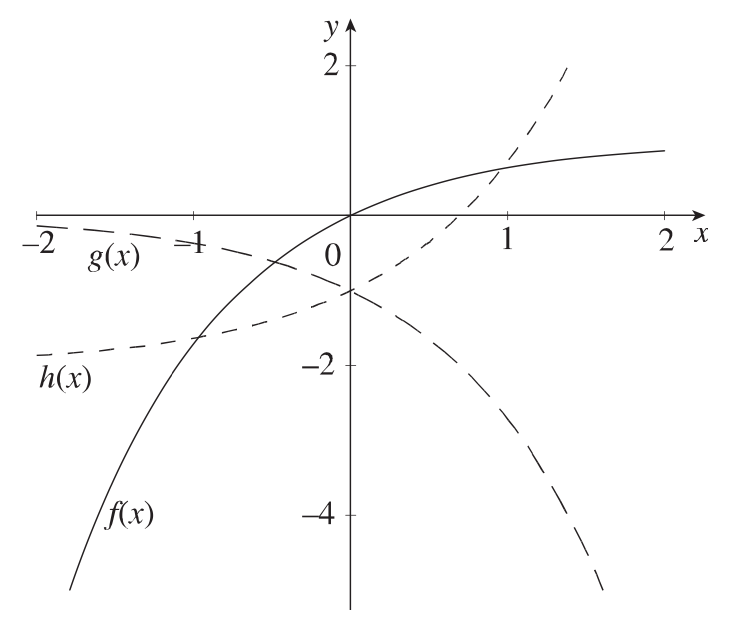
\includegraphics{Ch8s7-ws2-prob3.png}
\caption{}
Graph showing \(f(x)\): a concave down increasing function that passes through the origin, \(g(x)\): a concave down decreasing function that passes through the point \((0,-1)\), \(h(x)\): a concave up increasing function that passes through the point \((0,-1)\).%}
\end{figure}


\item  Find the series representations for the following functions by any means possible:

%\begin{multicols}{2}
\begin{enumerate}[(a)]

\item \(f(x) = \dfrac{1}{1+x^4}\)

\vspace*{1.5in}

%\item \(f(x) = \dfrac{1}{1+4x^2}\)
%
%\vspace*{.75in}
%
%\item \(f(x) = \ln\left|\dfrac{1+x}{1-x}\right|\)
%
%\vspace*{.75in}

\item \(f(x) = x^3 \sin x^2\)

\vspace*{1.5in}



\end{enumerate}

%\end{multicols}


%\item Let \(f(x) = \Sumzero a_n x^n\) and \(g(x) = \Sumzero b_n x^n\), with \(f(0) = g(0) = 0\).
%\begin{enumerate}[(a)]
%\item What does the condition \(f(0) = g(0) = 0\) mean in terms of the coefficients of the series?
%
%\vfill
%\item Compute \(\lim_{x\rightarrow 0} \frac{f(x)}{g(x)}\)
%\vfill
%
%\item Compute \(\lim_{x\rightarrow 0} \frac{\cos(x^2)-1}{\ln(1+x) - x}\) using the idea from part (b).

%\end{enumerate}

\end{enumerate}
\end{document}
